\documentclass[12pt]{article}
\usepackage{amsfonts,amssymb,float,amsmath}
\usepackage{algorithmic}
\usepackage{graphicx, siunintx}
\usepackage{textcomp}
\usepackage{xcolor}
\usepackage{txfonts}
\usepackage{multicol}
\usepackage{listings}
\usepackage{enumitem}
\usepackage{mathtools}
\usepackage{gensymb}
\usepackage{comment}
\usepackage[breaklinks=true]{hyperref}
\usepackage{tkz-euclide} 
\usepackage{listings}
\usepackage{gvv}                       
\usepackage{gvv-book}
%\def\inputGnumericTable{}                             
\usepackage{color}                                            
\usepackage{array}                                            
\usepackage{longtable}                                       
\usepackage{calc}                                             
\usepackage{multirow}                                         
\usepackage{hhline}                                           
\usepackage{ifthen}                                           
\usepackage{lscape}
\newcommand{\BEQA}{\begin{eqnarray}}
\newcommand{\EEQA}{\end{eqnarray}}
%\newcommand{\define}{\stackrel{\triangle}{=}}
\theoremstyle{remark}
\newtheorem{rem}{Remark}
\parindent 0px
\pagenumbering{gobble}
\begin{document}
\title{\vspace{-5cm}Gate paper 2023-XH}
\author{Ayush Sunil Labhade}
\date{AI25Btech11002}
\maketitle
\begin{flushright}Humanities and Social Sciences-English (XH-C2)\end{flushright} 
\begin{flushleft}General Aptitude \textbf{\brak{GA}} \\[5pt] 
\textbf{\item Q.1 - Q.5 Carry ONE mark each}\end{flushleft} 
\begin{enumerate}
%Q.1
\item Rafi told Mary, “I am thinking of watching a film this weekend.” 
The following reports the above statement in indirect speech:
Rafi told Mary that he \_\_\_\_\_\_\_ of watching a film that weekend. 
\begin{enumerate} \begin{multicols}{2}
\item thought 
\item is thinking 
\item am thinking 
\item was thinking 
\end{multicols} \end{enumerate}
\hfill\brak{GATE \ XH \ 2023}
%Q.2
\item Permit : \_\_\_\_\_\_\_ :: Enforce : Relax 
\brak{By word meaning}\newline 
\begin{enumerate} \begin{multicols}{4} 
\item Allow 
\item Forbid 
\item License 
\item Reinforce 
\end{multicols} \end{enumerate}
\hfill\brak{GATE \ XH \ 2023}
%Q.3
\item Given a fair six-faced dice where the faces are labelled ‘1’, ‘2’, ‘3’, ‘4’, ‘5’, and ‘6’,
what is the probability of getting a ‘1’ on the first roll of the dice and a ‘4’ on the
second roll? 
\begin{enumerate} \begin{multicols}{4}
\item $\frac{1}{36}$ 
\item $\frac{1}{6}$ 
\item $\frac{5}{6}$ 
\item $\frac{1}{3}$ 
\end{multicols} \end{enumerate}
\hfill\brak{GATE \ XH \ 2023}
%Q.4
\item A recent survey shows that 65% of tobacco users were advised to stop consuming
tobacco. The survey also shows that 3 out of 10 tobacco users attempted to stop
using tobacco. 
Based only on the information in the above passage, which one of the following
options can be logically inferred with certainty? 
\begin{enumerate}
\item A majority of tobacco users who were advised to stop consuming tobacco made an
attempt to do so. 
\item A majority of tobacco users who were advised to stop consuming tobacco did not
attempt to do so. 
\item Approximately 30% of tobacco users successfully stopped consuming tobacco. 
\item Approximately 65% of tobacco users successfully stopped consuming tobacco. 
\end{enumerate}
\hfill\brak{GATE \ XH \ 2023}
\newline
%Q.5
\item How many triangles are present in the given figure? 
\begin{centering}
\begin{figure}[H] 
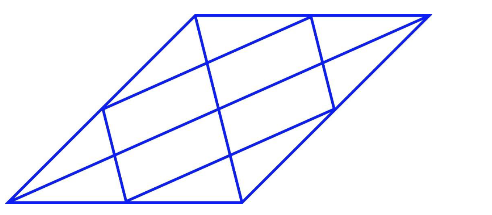
\includegraphics{Figs/Q5.png}
\caption{}
\label{Fig:1.1} 
\end{figure}
\end{centering}
\begin{enumerate} \begin{multicols}{4}
\item 12 
\item 16 
\item 20 
\item 24 
\end{multicols} \end{enumerate}
\hfill\brak{GATE \ XH \ 2023}
\newpage
\textbf{Q.6 - Q.10 Carry TWO marks Each} 
%Q.6
\item Students of all the departments of a college who have successfully completed the
registration process are eligible to vote in the upcoming college elections. However,
by the time the due date for registration was over, it was found that suprisingly none
of the students from the Department of Human Sciences had completed the
registration process. 
Based only on the information provided above, which one of the following sets of
statement(s) can be logically inferred with certainty? 
\begin{enumerate}
\item [(i)] All those students who would not be eligible to vote in the college elections
would certainly belong to the Department of Human Sciences. 
\item [(ii)] None of the students from departments other than Human Sciences failed to
complete the registration process within the due time. 
\item [(iii)] All the eligible voters would certainly be students who are not from the
Department of Human Sciences. 
\end{enumerate} 
\begin{enumerate} \begin{multicols}{4}
\item (i) and (ii) 
\item (i) and (iii) 
\item only (i) 
\item only (iii) 
\end{multicols} \end{enumerate}
\hfill\brak{GATE \ XH \ 2023}
%Q.7
\item Which one of the following options represents the given graph? 
\begin{figure}[H]
\centering
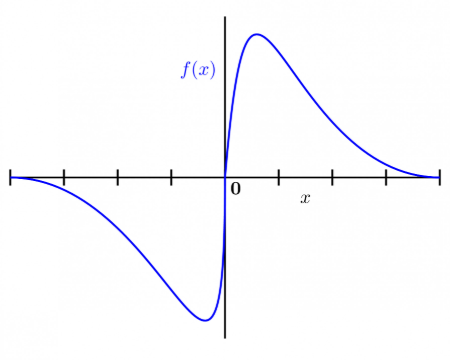
\includegraphics{Figs/Q7.png}
\caption{}
\label{Fig:1.2}
\end{figure}
\begin{enumerate} \begin{multicols}{4}
\item $f(x)=x^{2}2^{-|x|}$ 
\item $f(x)=x~2^{-|x|}$ 
\item $f(x)=|x|2^{-x}$ 
\item $f(x)=x~2^{-x}$ 
\end{multicols} \end{enumerate}
\hfill\brak{GATE \ XH \ 2023}
%Q.8
\item Which one of the options does NOT describe the passage below or follow from it? 
We tend to think of cancer as a ‘modern’ illness because its metaphors are
so modern. It is a disease of overproduction, of sudden growth, a growth
that is unstoppable, tipped into the abyss of no control. Modern cell biology
encourages us to imagine the cell as a molecular machine. Cancer is that
machine unable to quench its intial command (to grow) and thus transform
into an indestructible, self-propelled automaton. 
\sbrak{Adapted from The Emperor of All Maladies by Siddhartha Mukherjee} 
\begin{enumerate}
\item It is a reflection of why cancer seems so modern to most of us. 
\item It tells us that modern cell biology uses and promotes metaphors of machinery. 
\item Modern cell biology encourages metaphors of machinery, and cancer is often
imagined as a machine. 
\item Modern cell biology never uses figurative language, such as metaphors, to describe
or explain anything. 
\end{enumerate}
\hfill\brak{GATE \ XH \ 2023}
%Q.9
\item The digit in the unit’s place of the product $3^{999}\times7^{1000}$ is 
\begin{enumerate} \begin{multicols}{2}
\item 7 
\item 1 
\item 3 
\item 9 
\end{multicols} \end{enumerate}
\hfill\brak{GATE \ XH \ 2023}
%Q.10
\item A square with sides of length 6 cm is given. The boundary of the shaded region is
defined by two semi-circles whose diameters are the sides of the square, as shown. 
The area of the shaded region is \_\_\_\_ cm$^2$. 
\begin{figure}[H]
\centering
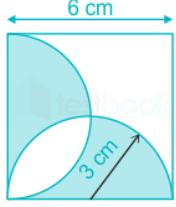
\includegraphics{Figs/Q10.png}
\caption{}
\label{Fig:1.3}
\end{figure} 
\begin{enumerate} \begin{multicols}{4} 
\item $6\pi$ 
\item 18 
\item 20 
\item $9\pi$ 
\end{multicols} \end{enumerate}
\hfill\brak{GATE \ XH \ 2023}
\newpage
\textbf{Reasoning and Comprehension – B1\newline 
XH-B1: Q.11 - Q.17 Carry ONE mark Each} 
%Q.11
\item Which word below best describes the idea of being both Spineless and Cowardly? 
\begin{enumerate} \begin{multicols}{2}
\item Pusillanimous 
\item Unctuous 
\item Obsequious 
\item Reticent 
\end{multicols} \end{enumerate}
\hfill\brak{GATE \ XH \ 2023}
%Q.12
\item Choose the right preposition to fill up the blank:
The whole family got together \_\_\_\_\_\_\_ Diwali 
\begin{enumerate} \begin{multicols}{4}
\item of 
\item at 
\item in 
\item till 
\end{multicols} \end{enumerate}
\hfill\brak{GATE \ XH \ 2023}
%Q.13
\item Select the correct option to fill in all the blanks to complete the passage: 
The (i) \_\_\_\_\_\_\_\_\_ factor amid this turbulence has been the (ii) \_\_\_\_\_\_\_\_\_ of high-
octane, action-oriented films such as RRR, K.G.F: Chapter 2 and Pushpa from film
industries in the south of the country. Traditionally, films made in the south have
done well in their own (iii) \_\_\_\_\_\_\_\_\_. But increasingly, their dubbed versions
have performed well in the Hindi heartland, with collections (iv) \_\_\_\_\_\_\_\_\_ those of
their Bollywood counterparts. 
\begin{enumerate} 
\item (i) disheartening (ii) failure (iii) channels (iv) matching 
\item (i) redeeming (ii) outperformance (iii) geographies (iv) eclipsing 
\item (i) shocking (ii) underperformance (iii) cinemas (iv) below 
\item (i) humbling (ii) bombing (iii) theatres (iv) falling behind 
\end{enumerate}
\hfill\brak{GATE \ XH \ 2023}
%Q.14
\item The following passage consists of 6 sentences. The first and sixth sentences of the
passage are at their correct positions, while the middle four sentences (represented
by 2, 3, 4, and 5) are jumbled up. 
Choose the correct sequence of the sentences so that they form a coherent
paragraph: 
\begin{enumerate}
\item[1.] Most obviously, mobility is taken to be a geographical as well as a social
phenomenon. 
\item[2.] Much of the social mobility literature regarded society as a uniform surface and
failed to register the geographical intersections of region, city and place, with
the social categories of class, gender and ethnicity. 
\item[3.] The existing sociology of migration is incidentally far too limited in its concerns
to be very useful here. 
\item[4.] Further, I am concerned with the flows of people within, but especially beyond,
the territory of each society, and how these flows may relate to many different
desires, for work, housing, leisure, religion, family relationships, criminal gain,
asylum seeking and so on. 
\item[5.] Moreover, not only people are mobile but so too are many 'objects'. 
\item[6.] I show that sociology’s recent development of a 'sociology of objects' needs to
be taken further and that the diverse flows of objects across societal borders and
their intersections with the multiple flows of people are hugely significant. 
\end{enumerate}
\begin{enumerate} \begin{multicols}{4}
\item 3, 2, 5, 4 
\item 2, 3, 4, 5 
\item 5, 4, 3, 2 
\item 4, 2, 5, 3 
\end{multicols} \end{enumerate}
\hfill\brak{GATE \ XH \ 2023}
%Q.15
\item The population of a country increased by 5% from 2020 to 2021. Then, the
population decreased by 5% from 2021 to 2022. By what percentage did the
population change from 2020 to 2022? 
\begin{enumerate} \begin{multicols}{4}
\item -0.25% 
\item 0% 
\item 2.5% 
\item 10.25% 
\end{multicols} \end{enumerate}
\hfill\brak{GATE \ XH \ 2023}
%Q.16
\item The words Thin: Slim: Slender are related in some way. Identify the correct
option(s) that reflect(s) the same relationship: 
\begin{enumerate} \begin{multicols}{2}
\item Fat: Plump: Voluptuous 
\item Short: Small: Petite 
\item Tall: Taller: Tallest 
\item Fair: Dark: Wheatish 
\end{multicols} \end{enumerate}
\hfill\brak{GATE \ XH \ 2023}
%Q.17
\item A pandemic like situation hit the country last year, resulting in loss of human life
and economic depression. To improve the condition of its citizens, the government
made a series of emergency medical interventions and increased spending to revive
the economy. In both these efforts, district administration authorities were actively
involved. 
Which of the following action(s) are plausible? 
\begin{enumerate}
\item In future, the government can make district administration authorities responsible
for protecting health of citizens and reviving the economy. 
\item The government may set up a task force to review the post pandemic situation and
ascertain the effectiveness of the measures taken. 
\item The government may set up a committee to formulate a pandemic management
program to minimize losses to life and economy in future. 
\item The government may take population control measures to minimize pandemic
related losses in future. 
\end{enumerate}
\hfill\brak{GATE \ XH \ 2023}
\newpage
\textbf{XH-B1: Q.18 - Q.26 Carry TWO marks Each} 
%Q.18
\item Six students, Arif, Balwinder, Chintu, David, Emon and Fulmoni appeared in the
GATE-XH exam in 2022. Balwinder scores less than Chintu in XH-B1, but more
than Arif in XH-C1. David scores more than Balwinder in XH-C1, and more than
Chintu in XH-B1. Emon scores less than David, but more than Fulmoni in XH-B1.
Fulmoni scores more than David in XH-C1. Arif scores less than Emon, but more
than Fulmoni in XH-B1. Who scores highest in XH-B1? 
\begin{enumerate} \begin{multicols}{4}
\item Fulmoni 
\item Emon 
\item David 
\item Chintu 
\end{multicols} \end{enumerate}
\hfill\brak{GATE \ XH \ 2023}
%Q.19
\item Select the correct relation between E and F. 
$$ E=\frac{x}{1+x} \text{ and } F=\frac{-x}{1-x} \text{ where } x>1 $$ 
\begin{enumerate} \begin{multicols}{4}
\item $E>F$ 
\item $E<F$ 
\item $E=F$ 
\item $E<-F$ 
\end{multicols} \end{enumerate}
\hfill\brak{GATE \ XH \ 2023}
%Q.20
\item A code language is formulated thus:
Vowels in the original word are replaced by the next vowel from the list of vowels,
A-E-I-O-U (For example, E is replaced by I and U is replaced by A). Consonants
in the original word are replaced by previous consonant (For example, T is
replaced by S and V is replaced by T). 
Then how does the word, GOODMORNING appear in the coded language? 
\begin{enumerate} \begin{multicols}{2}
\item HUUFNUSPOPH 
\item FIICLIQMEMF 
\item FUUCLUQMOMF 
\item HEEDATTACRH 
\end{multicols} \end{enumerate}
\hfill\brak{GATE \ XH \ 2023}
%Q.21
\item The stranger is by nature no ""owner of soil"" -- soil not only in the physical, but also
in the figurative sense of a life-substance, which is fixed, if not in a point in space,
at least in an ideal point of the social environment. Although in more intimate
relations, he may develop all kinds of charm and significance, as long as he is
considered a stranger in the eyes of the other, he is not an ""owner of soil.""
Restriction to intermediary trade, and often (as though sublimated from it) to pure
finance, gives him the specific character of mobility. If mobility takes place within
a closed group, it embodies that synthesis of nearness and distance which constitutes
the formal position of the stranger. For, the fundamentally mobile person comes in
contact, at one time or another, with every individual, but is not organically
connected, through established ties of kinship, locality, and occupation, with any
single one. 
What assumptions can be made about the stranger from the passage above? 
\begin{enumerate}
\item The stranger can become an owner of soil through developing all kinds of charm in
more intimate relations. 
\item The stranger cannot become an owner of soil either in the physical or psychological
sense. 
\item The stranger can become an owner of soil through establishing ties of kinship and
so on. 
\item The stranger might become an owner of soil in the physical sense but not in the
psychological 
\end{enumerate}
\hfill\brak{GATE \ XH \ 2023}
%Q.22
\item L is the only son of A and S. S has one sibling, B, who is married to L's aunt, K.
B is the only son of D. How are L and D related?
Select the possible option(s): 
\begin{enumerate}
\item Grandchild and Paternal Grandfather 
\item Grandchild and Maternal Grandfather 
\item Grandchild and Paternal Grandmother 
\item Grandchild and Maternal Grandmother 
\end{enumerate}
\hfill\brak{GATE \ XH \ 2023}
%Q.23
\item Five segments of a sentence are given below. The first and fifth segments are at
their correct positions, while the middle three segments (represented by 2, 3, and 4)
are jumbled up. Choose the correct order of the segments so that they form a
coherent sentence: 
\begin{enumerate}
\item[1.] Consumed multitudes are jostling and shoving inside me 
\item[2.] and guided only by the memory of a large white bedsheet with a roughly
circular hole some seven inches in diameter cut into the center, 
\item[3.] clutching at the dream of that holey, mutilated square of linen, which is my
talisman, my open-sesame, 
\item[4.] I must commence the business of remaking my life from the point at which
it really began, 
\item[5.] some thirty-two years before anything as obvious, as present, as my clock-
ridden, crime-stained birth. 
\end{enumerate}
\begin{enumerate} \begin{multicols}{4}
\item $2-3-4$ 
\item $3-2-4$ 
\item $4-2-3$ 
\item $4-3-2$ 
\end{multicols} \end{enumerate}
\hfill\brak{GATE \ XH \ 2023}
%Q.24
\item “I told you the truth,” I say yet again, “Memory’s truth, because memory has its
own special kind. It selects, eliminates, alters, exaggerates, minimizes, glorifies, and
vilifies also; but in the end it creates its own reality, its heterogeneous but usually
coherent versions of events; and no sane human being ever trusts someone else’s
version more than his own.” 
What are the different ways in which ‘truth’ can be understood from the passage? 
\begin{enumerate}
\item Truth is what can be verified by hard empirical evidence. 
\item Truth is based on what can be perceived by the senses. 
\item Truth is the product of memory that is fallible, selective and slanted. 
\item Truth is contingent on the observer and can only be partial. 
\end{enumerate}
\hfill\brak{GATE \ XH \ 2023}
%Q.25
\item A firm needs both skilled labour and unskilled labour for the production of cloth.
The wage of skilled labour is Rs. 40,000 per month, and that of unskilled labour is
Rs. 15,000 per month. The total wage bill of the firm for the production of cloth is
Rs. 23,75,000 in a month for 100 labour. How many skilled labour are employed
by the firm (in Integer)? 
\hfill\brak{GATE \ XH \ 2023}
%Q.26
\item Select the odd word and write the option number as answer: 
(1) Lek (2) Zloty (3) Diner (4) Drachma (5) Real 
\hfill\brak{GATE \ XH \ 2023}
\newpage
\textbf{English - C2 \newline 
XH-C2: Q.27-Q.44 Carry ONE mark Each} 
%Q.27
\item Who published the novel The Bell Jar under the pseudonym Victoria Lucas? 
\begin{enumerate} \begin{multicols}{2}
\item Dorothy Richardson 
\item Virginia Woolf 
\item Sylvia Plath 
\item Alice Walker 
\end{multicols} \end{enumerate}
\hfill\brak{GATE \ XH \ 2023}
%Q.28
\item In which collection did Walt Whitman's poem ""Song of Myself"" first appear? 
\begin{enumerate} \begin{multicols}{2}
\item Two Rivulets 
\item November Boughs 
\item The Golden Bough 
\item Leaves of Grass 
\end{multicols} \end{enumerate}
\hfill\brak{GATE \ XH \ 2023}
%Q.29
\item Who wrote the introduction to Rabindranath Tagore's Gitanjali? 
\begin{enumerate} \begin{multicols}{2}
\item T. S. Eliot 
\item Ezra Pound 
\item W. H. Auden 
\item W. B. Yeats 
\end{multicols} \end{enumerate}
\hfill\brak{GATE \ XH \ 2023}
%Q.30
\item Identify the title of the poem in which the following lines appear: 
""He was found by the Bureau of Statistics to be
One against whom there was no official complaint,
And all the reports on his conduct agree
That, in the modern sense of an old-fashioned word, he was a saint
For in everything he did he served the greater community."" 
\begin{enumerate} 
\item ""In Memory of W. B. Yeats"" 
\item ""The Unknown Citizen"" 
\item ""In Praise of Limestone"" 
\item ""On this Island"" 
\end{enumerate}
\hfill\brak{GATE \ XH \ 2023}
%Q.31
\item Identify the point of view used in the following passage:
""You are not the kind of guy who would be at a place like this at this time of the
morning. But here you are, and you cannot say that the terrain is entirely
unfamiliar, though the details are fuzzy."" 
\begin{enumerate} 
\item Third-person point of view 
\item The limited point of view 
\item Second-person point of view 
\item First-person point of view 
\end{enumerate}
\hfill\brak{GATE \ XH \ 2023}
%Q.32
\item Which of the following is a novel by Charles Dickens? 
\begin{enumerate} \begin{multicols}{2}
\item The Old Curiosity Shop 
\item The Old Wives' Tale 
\item The Old Bachelor 
\item One Hundred Years of Solitude 
\end{multicols} \end{enumerate}
\hfill\brak{GATE \ XH \ 2023}
%Q.33
\item Which linguistic process can be seen in the formation of the following words?
i. smog, ii. brunch, iii. motel iv. telecast 
\begin{enumerate} \begin{multicols}{2}
\item Borrowing 
\item Compounding 
\item Blending 
\item Backformation 
\end{multicols} \end{enumerate}
\hfill\brak{GATE \ XH \ 2023}
%Q.34
\item Which writer is credited with the 'chutneyfication' of Indian English? 
\begin{enumerate} \begin{multicols}{2}
\item Raja Rao 
\item Salman Rushdie 
\item Amitav Ghosh 
\item Arundhati Roy 
\end{multicols} \end{enumerate}
\hfill\brak{GATE \ XH \ 2023}
%Q.35
\item Whom would you associate the term 'simulacra' with? 
\begin{enumerate} \begin{multicols}{2}
\item Noam Chomsky 
\item Jean Baudrillard 
\item Félix Guattari 
\item Michel Foucault 
\end{multicols} \end{enumerate}
\hfill\brak{GATE \ XH \ 2023}
%Q.36
\item In Plato's idea of the Republic there is no place for the 
\begin{enumerate} \begin{multicols}{4}
\item Lawyer 
\item Magistrate 
\item Politician 
\item Poet 
\end{multicols} \end{enumerate}
\hfill\brak{GATE \ XH \ 2023}
%Q.37
\item What was Aristotle's definition of hubris? 
\begin{enumerate} 
\item Tragic flaw in a character 
\item A false sense of pride which eventually causes the character's downfall 
\item An ability to imagine the future 
\item A humble, ascetic quality 
\end{enumerate}
\hfill\brak{GATE \ XH \ 2023}
%Q.38
\item Stephen Dedalus is a recurring character in the works of 
\begin{enumerate} \begin{multicols}{4}
\item James Joyce 
\item H. G. Wells 
\item P. G. Wodehouse 
\item D. H. Lawrence 
\end{multicols} \end{enumerate}
\hfill\brak{GATE \ XH \ 2023}
%Q.39
\item Which of the following novels opens with the sentence, ""It is a truth universally
acknowledged that a single man in possession of a good fortune must be in want
of a wife.""? 
\begin{enumerate} \begin{multicols}{2}
\item Sense and Sensibility 
\item Pride and Prejudice 
\item Mansfield Park 
\item Emma 
\end{multicols} \end{enumerate}
\hfill\brak{GATE \ XH \ 2023}
%Q.40
\item Which of the following novels by Chinua Achebe derives its title from W. B.
Yeats's poem ""The Second Coming""? 
\begin{enumerate} \begin{multicols}{2}
\item Arrow of God 
\item No Longer at Ease 
\item A Man of the People 
\item Things Fall Apart 
\end{multicols} \end{enumerate}
\hfill\brak{GATE \ XH \ 2023}
%Q.41
\item Identify the novels that deal with the trauma of Partition: 
\begin{enumerate} 
\item Shauna Singh Baldwin's What the Body Remembers 
\item Amitav Ghosh's The Shadow Lines 
\item Anita Desai's Cry, the Peacock 
\item Kamala Markandaya's Nectar in a Sieve 
\end{enumerate}
\hfill\brak{GATE \ XH \ 2023}
%Q.42
\item Which of the following writers are associated with the Theatre of the Absurd? 
\begin{enumerate} \begin{multicols}{2}
\item Harold Pinter 
\item Edward Albee 
\item John Osborne 
\item Eugene O'Neill 
\end{multicols} \end{enumerate}
\hfill\brak{GATE \ XH \ 2023}
%Q.43
\item Identify the writers who are referred to as 'metaphysical poets': 
\begin{enumerate} \begin{multicols}{2}
\item John Donne 
\item Andrew Marvell 
\item Philip Larkin 
\item T. S. Eliot 
\end{multicols} \end{enumerate}
\hfill\brak{GATE \ XH \ 2023}
%Q.44
\item What are the sources of Girish Karnad's Hayavadana? 
\begin{enumerate} 
\item Thomas Mann's The Transported Heads 
\item Valmiki's Ramayana 
\item Somadeva's Kathasaritsagara 
\item Franz Kafka's The Metamorphosis 
\end{enumerate}
\hfill\brak{GATE \ XH \ 2023}
\newpage
\textbf{XH-C2: Q.45-Q.65 Carry TWO marks Each} 
%Q.45
\item Which of the following terms are used by Samuel Taylor Coleridge in his theory
of imagination? 
\begin{enumerate} 
\item Primary imagination, secondary imagination, and fancy 
\item Negative capability, Hellenism, and impersonality 
\item Egotistical sublime, oversoul, and pantheism 
\item Unacknowledged legislation, atheism, and anarchy 
\end{enumerate}
\hfill\brak{GATE \ XH \ 2023}
%Q.46
\item Which of the following is the forerunner of the autobiography? 
\begin{enumerate} 
\item St. Augustine's Confessions 
\item James Joyce's Portrait of the Artist as a Young Man 
\item William Wordsworth's The Prelude 
\item Izaak Walton's Lives 
\end{enumerate}
\hfill\brak{GATE \ XH \ 2023}
%Q.47
\item Which of the following poems did Robert Browning intend to write as a play? 
\begin{enumerate} \begin{multicols}{2}
\item ""Men and Women"" 
\item ""Dramatis Personae"" 
\item ""The Inn Album"" 
\item ""The Ring and the Book"" 
\end{multicols} \end{enumerate}
\hfill\brak{GATE \ XH \ 2023}
%Q.48
\item The 'Age of Reason' in English literary history is popularly known as: 
\begin{enumerate} \begin{multicols}{2}
\item The Medieval Period 
\item The Neo-classical Age 
\item The Romantic Age 
\item The Victorian Age 
\end{multicols} \end{enumerate}
\hfill\brak{GATE \ XH \ 2023}
%Q.49
\item Who first translated Jacques Derrida's work into English? 
\begin{enumerate} \begin{multicols}{2}
\item Gayatri C. Spivak 
\item Edward Said 
\item Harold Bloom 
\item Paul de Man 
\end{multicols} \end{enumerate}
\hfill\brak{GATE \ XH \ 2023}
%Q.50
\item Identify the 'Lake Poets': 
\begin{enumerate} 
\item Byron, Shelley, Keats 
\item Wordsworth, Coleridge, Byron 
\item Byron, Southey, Wordsworth 
\item Wordsworth, Coleridge, Southey 
\end{enumerate}
\hfill\brak{GATE \ XH \ 2023}
%Q.51
\item Choose from the following options the type of drama that is intended by the
author to be read rather than to be performed: 
\begin{enumerate} \begin{multicols}{2}
\item Kitchen Sink Drama 
\item Closet Drama 
\item Poetic Drama 
\item Folk Drama 
\end{multicols} \end{enumerate}
\hfill\brak{GATE \ XH \ 2023}
%Q.52
\item Identify the commonality shared by the authors of Mansfield Park and Middle
March: 
\begin{enumerate} 
\item Both the novels were authored by men who were sent on exile. 
\item Both the novels were authored by political prisoners. 
\item Both the novels were written by children who were not allowed to publish their
works. 
\item Both the novels were written by women who wrote under pseudonyms. 
\end{enumerate}
\hfill\brak{GATE \ XH \ 2023}
%Q.53
\item Who said, ""Poetry makes nothing happen""? 
\begin{enumerate} \begin{multicols}{2}
\item Marianne Moore 
\item Ezra Pound 
\item Wallace Stevens 
\item W. H. Auden 
\end{multicols} \end{enumerate}
\hfill\brak{GATE \ XH \ 2023}
%Q.54
\item Which literary device does the following line employ?
""A timorous foe, and a suspicious friend."" 
\begin{enumerate} \begin{multicols}{4}
\item Antithesis 
\item Antistrophe 
\item Oxymoron 
\item Apostrophe 
\end{multicols} \end{enumerate}
\hfill\brak{GATE \ XH \ 2023}
%Q.55
\item Match the following excerpts with their authors: 
\begin{table}[H]
\begin{tabular}{|p{3in}|p{1.5in}|}
\hline
(P) ""He rose from the table; and advancing to the master, basin and spoon in hand, said: somewhat alarmed at his own temerity: 'Please, Sir, I want some more."" & (i) Ralph Waldo Emerson \\
\hline
(Q) ""Studies serve for delight, for ornament, and for ability."" & (ii) George Orwell \\
\hline
(R) ""Trust thyself: every heart vibrates to that iron string."" & (iii) Charles Dickens \\
\hline
(S) ""It was a bright cold day in April, and the clocks were striking thirteen."" & (iv) Francis Bacon \\
\hline
\end{tabular}

\caption{}
\label{Table 1.1}
\end{table}
\begin{enumerate}
\item (P)-(iii), (Q)-(iv), (R)-(i), (S)-(ii) 
\item (P)-(iv), (Q)-(iii), (R)-(ii), (S)-(i) 
\item (P)-(iii), (Q)-(ii), (R)-(i), (S)-(iv) 
\item (P)-(i), (Q)-(iv), (R)-(ii), (S)-(iii) 
\end{enumerate}
\hfill\brak{GATE \ XH \ 2023}
%Q.56
\item The 1667 edition of Paradise Lost had 10 books. How many more were added to
the 1674 edition? 
\begin{enumerate} \begin{multicols}{4}
\item 2 
\item 4 
\item 6 
\item 12 
\end{multicols} \end{enumerate}
\hfill\brak{GATE \ XH \ 2023}
%Q.57
\item Read the following poem and identify the appropriate options: 
"And search
for certain thin
stemmed, bubble-eyed water bugs.
See them perch
on dry capillary legs
weightless
on the ripple skin
of a stream.
No, not only prophets
walk on water. This bug sits
on a landslide of lights
and drowns eye
deep
into its tiny strip
of sky." 
\begin{enumerate}
\item It uses free verse form. 
\item It employs imagery. 
\item It uses the iambic pentameter. 
\item It juxtaposes the non-human with the human. 
\end{enumerate}
\hfill\brak{GATE \ XH \ 2023}
%Q.58
\item Which of the following employ 'Interior Monologue'? 
\begin{enumerate} 
\item Alfred Lord Tennyson's ""In Memoriam"" 
\item The final chapter of James Joyce's Ulysses 
\item T. S. Eliot's ""The Love Song of J. Alfred Prufrock"" 
\item Robert Browning's ""My Last Duchess"" 
\end{enumerate}
\hfill\brak{GATE \ XH \ 2023}
%Q.59
\item Which of the following works may be described as novels in verse? 
\begin{enumerate} 
\item Aurora Leigh by Elizabeth Barrett Browning 
\item The Golden Gate by Vikram Seth 
\item Pamela by Samuel Richardson 
\item Old Possum's Book of Practical Cats by T. S. Eliot 
\end{enumerate}
\hfill\brak{GATE \ XH \ 2023}
%Q.60
\item Which of the following critics belong to the deconstructionist school? 
\begin{enumerate} \begin{multicols}{2} 
\item Jacques Derrida 
\item Paul de Man 
\item J. Hillis Miller 
\item Kate Soper 
\end{multicols} \end{enumerate}
\hfill\brak{GATE \ XH \ 2023}
%Q.61
\item Cleanth Brooks's definition of 'paradox' in poetry foregrounds the following
qualities: 
\begin{enumerate} 
\item Wonder and irony 
\item Contradiction and qualification 
\item Piety and plurality 
\item Omniscience and death of the author 
\end{enumerate}
\hfill\brak{GATE \ XH \ 2023}
%Q.62
\item Two examples of magic realist fiction include: 
\begin{enumerate} \begin{multicols}{2}
\item Midnight's Children 
\item The Tin Drum 
\item The English Teacher 
\item Tom Jones 
\end{multicols} \end{enumerate}
\hfill\brak{GATE \ XH \ 2023}
%Q.63
\item Ferdinand de Saussure differentiates language in terms of: 
\begin{enumerate} \begin{multicols}{4} 
\item langue 
\item metaphor 
\item metonymy 
\item parole 
\end{multicols} \end{enumerate}
\hfill\brak{GATE \ XH \ 2023}
%Q.64
\item Which of the following are considered to be typical postmodern narratives? 
\begin{enumerate} 
\item Italo Calvino's If on a Winter's Night a Traveller 
\item John Barth's Lost in the Funhouse 
\item Thomas Pynchon's V. 
\item Iris Murdoch's The Bell 
\end{enumerate}
\hfill\brak{GATE \ XH \ 2023}
%Q.65
\item What does a green reading of a text aim at? 
\begin{enumerate} 
\item Analyzing the implications of a text for environmental concerns 
\item Deconstructing human exceptionalism 
\item Studying connections between humans, society and the non-human world 
\item Marginalizing differently abled people 
\end{enumerate}
\hfill\brak{GATE \ XH \ 2023}
\end{enumerate}
\end{document}
